\documentclass[11pt]{article}

\usepackage[margin=1in]{geometry}
\usepackage{array}
\usepackage{booktabs}
\usepackage{float}
\usepackage{hyperref}
\usepackage{microtype}
\usepackage{tikz}
\usepackage{xcolor}
\usetikzlibrary{arrows.meta, positioning, calc}
\setlength{\emergencystretch}{3em}
\renewcommand{\arraystretch}{1.18}

\definecolor{ocoTeal}{HTML}{63C3BA}
\definecolor{ocoBlue}{HTML}{5F8FD3}
\definecolor{ocoOrange}{HTML}{E97755}
\definecolor{ocoGray}{HTML}{EDEDED}
\definecolor{ocoDark}{HTML}{222222}
\definecolor{ocoMute}{HTML}{8C9098}
\definecolor{scaleSky}{HTML}{6EC7E8}
\definecolor{scaleSalmon}{HTML}{E97755}
\definecolor{scalePurple}{HTML}{5F8FD3}
\definecolor{scalePink}{HTML}{D86BB0}

\title{Harness and Serving-Profile Effects on SWE-bench Pro:\\
An Evidence-First Case Study with OpenCodeOrchestra and Qwen3.6-27B}
\author{Aiden Kim}
\date{Technical report --- May 2026}

\begin{document}
\maketitle

\begin{abstract}
Repository-level coding-agent scores measure complete runtime systems, not model weights alone. This report studies OpenCodeOrchestra (OCO), an opencode-based harness organized around a Project Manager $\rightarrow$ Orchestrator $\rightarrow$ specialist-agent workflow, on SWE-bench Pro with open-weight Qwen3.6-27B. A seeded-subset pilot served on a non-speculative Runpod B200 profile resolved 162/223 submitted patch rows (72.6\% strict, Wilson 95\% CI 66.4--78.1\%). A later 731-task H200 FP8 + MTP-4 run with a different controller collapsed to 28.45\% strict; replaying the B200 patches through the same evaluator reproduced the high result. The systems lesson is direct: faster serving is not automatically better serving for long-horizon coding agents.
\end{abstract}

\section{Introduction}

A repository-level coding agent must inspect a codebase, interpret an issue, edit source, reason about tests, and submit a patch accepted by an external evaluator. The surrounding runtime---prompt hierarchy, tools, permissions, retry policy, patch extraction, and model-serving stack---changes the outcome.

This report studies that systems problem through OpenCodeOrchestra (OCO), a durable orchestration harness for software-engineering tasks. The contribution is an audited artifact trail showing (i) a strong seeded-subset pilot under an archived B200 non-speculative profile, (ii) transparent denominator accounting, and (iii) a later deployment-profile collapse caused by worse generated patches rather than evaluator failure.

The rule used throughout is: source artifacts are the evidence. Chat transcripts are pointers only. Load-bearing claims are tied to checked-in source, archived runner source, manifests, evaluator outputs, replay roots, and forensic notes.

\paragraph{Contributions.}
\begin{enumerate}
  \item A deterministic, repository-balanced seeded-subset pilot on SWE-bench Pro with transparent denominators.
  \item An OCO harness configuration where PM-to-Orchestrator delegation was broadly observed and Auditor participation was available but not consistently enforced.
  \item Validation of the positive patch bundle through replay on the later Modal/evaluator stack and manual inspection of representative passing histories.
  \item A negative serving/controller-profile result: token-throughput wins and full-patch generation do not guarantee task-level coding-agent quality.
\end{enumerate}

\section{Background and Related Work}

\paragraph{Repository-level coding benchmarks.}
SWE-bench shifted coding-agent evaluation from short programming problems toward real GitHub issue resolution \cite{jimenez2024swebench}. SWE-bench Verified introduced a human-filtered subset intended to reduce ambiguous tasks \cite{swebenchverified2024}. SWE-bench Pro extends the family toward longer-horizon, industrial repository tasks \cite{deng2025swebenchpro}. Task selection, evaluator version, bundle shape, and runtime budget are methodology variables, not incidental details.

\paragraph{Harness and agent-computer-interface effects.}
SWE-agent argued that the agent-computer interface is itself an experimental object: the same language model performs differently depending on observations, actions, shell/editor affordances, and submit loops \cite{yang2024sweagent}. mini-SWE-agent shows a compact scaffold can be strong and reproducible when the interface is clean \cite{sweagent2025minisweagent}. Agentless shows that autonomous tool use is not automatically the winning variable; structured localization, repair, and validation can compete with more complex loops \cite{xia2025agentless}. OpenHands provides a broad open platform for sandboxed software agents \cite{wang2025openhands}. OCO belongs in this line of work: the harness is part of the treatment.

\paragraph{Multi-agent software-engineering systems.}
MetaGPT and ChatDev organized software work into teams of named roles \cite{hong2024metagpt,qian2024chatdev}. Repository-repair systems such as MAGIS, CodeR, and HyperAgent explore manager/developer/QA or task-graph decompositions \cite{tao2024magis,chen2024coder,phan2024hyperagent}. OCO contributes a concrete runtime: persistent Orchestrator sessions, task-local specs, permissioned specialists, context-compression tooling, and audit-oriented workflow concepts built into a production fork of opencode.

\paragraph{Reviewer, verifier, and audit loops.}
Verifier and reviewer loops can improve code-generation systems when enforced and measured. OCO includes an Auditor concept; the positive bundle contains an audit-observed stratum. In this pilot, audit is a harness capability and observability variable; the measured treatment is the broader OCO runtime.

\paragraph{Serving-profile sensitivity.}
Inference serving is an underreported variable in coding-agent studies. Quantization, KV-cache format, context length, batching, parser behavior, and speculative decoding can change more than throughput. A direct server-throughput A/B favored an H200 FP8 + MTP-4 profile, but downstream full-task generation quality collapsed. Because old patches replayed successfully through the same evaluator while new patches failed by ordinary code-quality mechanisms, the case study motivates task-level quality A/B tests for serving profiles.

\section{System Under Measurement: OpenCodeOrchestra}

OCO extends opencode with a Project Manager $\rightarrow$ Orchestrator $\rightarrow$ specialist-agent workflow. PM gathers context and writes a task-local spec; Orchestrator owns implementation; Investigator and Auditor support evidence gathering and review. OCO source: \url{https://github.com/AidenGeunGeun/OpenCodeOrchestra} \cite{kim2026opencodeorchestra}. The benchmarked setup used OCO as an installed CLI; the benchmark repository does not modify OCO source.

\begin{figure}[H]
\centering
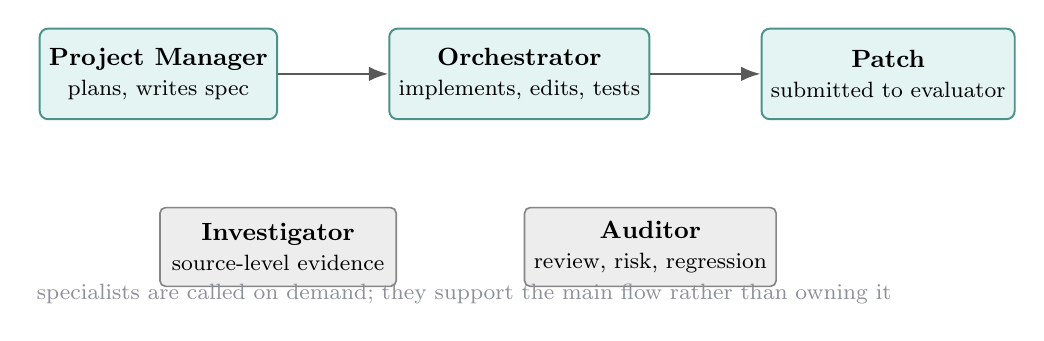
\begin{tikzpicture}[
  node distance=1.1cm and 1.4cm,
  primary/.style={draw, rounded corners=3pt, minimum width=3.0cm, minimum height=1.15cm, align=center, font=\small, fill=ocoTeal!18, draw=ocoTeal!75!black, line width=0.7pt},
  specialist/.style={draw, rounded corners=2pt, minimum width=3.0cm, minimum height=1.0cm, align=center, font=\small, fill=ocoGray, draw=ocoDark!55, line width=0.6pt},
  flow/.style={-Latex, line width=0.9pt, draw=ocoDark!75}
]
\node[primary] (pm) {\textbf{Project Manager}\\\footnotesize plans, writes spec};
\node[primary, right=of pm] (orch) {\textbf{Orchestrator}\\\footnotesize implements, edits, tests};
\node[primary, right=of orch] (patch) {\textbf{Patch}\\\footnotesize submitted to evaluator};
\draw[flow] (pm) -- (orch);
\draw[flow] (orch) -- (patch);

\node[specialist, below=1.1cm of pm.south east, xshift=-0.0cm] (inv) {\textbf{Investigator}\\\footnotesize source-level evidence};
\node[specialist, below=1.1cm of orch.south east, xshift=0.0cm] (aud) {\textbf{Auditor}\\\footnotesize review, risk, regression};
\node[font=\footnotesize, text=ocoMute, below=0.35cm of $(inv)!0.5!(aud)$] {specialists are called on demand; they support the main flow rather than owning it};
\end{tikzpicture}
\caption{OCO workflow. PM owns task framing; Orchestrator owns implementation. Investigator and Auditor are support roles rather than extra implementation owners.}
\label{fig:arch}
\end{figure}

\begin{center}
\begin{tabular}{p{0.27\linewidth}p{0.60\linewidth}}
\toprule
Component & Measured status in the positive pilot \\
\midrule
PM $\rightarrow$ Orchestrator delegation & Broadly observed across the 223 clean rows; archived methodology reports all 223 had an observed Orchestrator task/session and 221 had delegation-like snippets. \\
Auditor loop & Available and prompted, not consistently enforced; archived split: 37 audit-observed, 185 audit-missing, 1 absence-justified. \\
Durable handoff back to PM & Often absent because resumed Orchestrator contexts frequently lacked the durable handoff tool; treated as telemetry caveat, not patch failure. \\
Direct PM edits & Common and recorded; representativeness warning for strict PM/Orchestrator separation. \\
Benchmark boundary & The benchmark consumes an installed OCO CLI and must not patch OCO source. \\
\bottomrule
\end{tabular}
\par\vspace{0.5em}
\small\textbf{Table 1.} What was actually measured in the positive pilot.
\end{center}

\section{Experimental Protocol and Evidence Chain}

\begin{figure}[H]
\centering
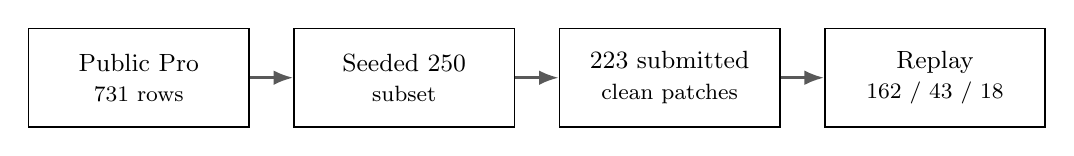
\begin{tikzpicture}[
  node distance=0.55cm,
  stage/.style={draw, rectangle, minimum height=1.25cm, minimum width=2.8cm, align=center, font=\small, line width=0.6pt, fill=white},
  flow/.style={-Latex, line width=0.9pt, draw=ocoDark!75}
]
\node[stage] (a) {Public Pro\\\footnotesize 731 rows};
\node[stage, right=of a] (b) {Seeded 250\\\footnotesize subset};
\node[stage, right=of b] (c) {223 submitted\\\footnotesize clean patches};
\node[stage, right=of c] (d) {Replay\\\footnotesize 162 / 43 / 18};
\draw[flow] (a) -- (b);
\draw[flow] (b) -- (c);
\draw[flow] (c) -- (d);
\end{tikzpicture}
\caption{Evidence chain for the positive pilot. Each arrow is backed by an archived source artifact: controller pinning, seeded selection report, final bundle manifest, and current-evaluator replay outputs.}
\label{fig:chain}
\end{figure}

\subsection{Task source and public split}
The current controller pins SWE-bench Pro to \path{ScaleAI/SWE-bench_Pro}, split \texttt{test}, revision \texttt{7ab5114912baf22bb098818e604c02fe7ad2c11f}. It records the expected public split size of 731 rows, canonicalizes required fields, sorts by instance id, and writes SHA-256 manifests. This is not retroactive proof of the earlier pilot, but it defines the cleaned artifact standard now used by the repository.

\subsection{Seeded 250-task subset}
The positive pilot used a deterministic, repository-balanced subset. The archived runner grouped rows by repository, sorted rows within each repository by SHA-256 digest, sorted repositories by SHA-256 digest, then round-robined across repositories. The final seeded-250 pilot was the first 250 rows of a previously materialized full-731 order produced by that procedure. The archived preparation report records \texttt{selected\_count=250}, \texttt{source\_count=731}, selected IDs, per-repository counts, and the method string. The subset is repository-balanced but not category-balanced or deduplicated.

\subsection{Positive-pilot serving profile}
The archived positive run id is \texttt{qwen36-pro-full731-oco-b200-guarded-c5-20260520T050248Z}. The archived final methodology note identifies a Runpod B200 pod serving \texttt{Qwen/Qwen3.6-27B-FP8}, with 262,144-token server context, prefix caching, Qwen reasoning parser, non-streaming tool calls, and no speculative decoding. Metrics summaries record no speculative-acceptance counters.

Some later notes and replay-directory names call the positive bundle ``NVFP4.'' This report follows the archived final methodology note for the quantization label and treats the mismatch as an artifact-labeling caveat.

\subsection{Evaluation path and replay}
The final positive bundle contained 223 submitted clean patch rows and 223 matching raw rows out of the 250 selected tasks; the manifest records 27 excluded selected attempts with reasons. The bundle was later replayed through the current Modal/SWE-bench Pro evaluator checkout used for the H200 full-run evaluation. Parsing replay outputs gave \textbf{162 pass, 43 fail, 18 empty-test outputs} over 223 rows. The original archived combined tally was 158 / 46 / 19; this report uses 162/223 for current-evaluator comparability and discloses the historical archive tally alongside.

\subsection{Denominator flow}
\begin{center}
\begin{tabular}{p{0.34\linewidth}rp{0.43\linewidth}}
\toprule
Stage & Count & Evidence / interpretation \\
\midrule
Seeded subset & 250 & Deterministic repository-balanced subset from the public 731-row order. \\
Submitted clean patch rows & 223 & Clean patches with matching raw rows in the final bundle manifest. \\
Excluded selected attempts & 27 & Infrastructure artifacts, invalid orchestration, empty/missing patches, dependency setup failure; not submitted. \\
Replay pass & 162 & Parsed as resolved in the current Modal/evaluator replay. \\
Replay fail & 43 & Meaningful evaluator non-pass among submitted rows. \\
Replay empty-test outputs & 18 & Manually inspected: mostly real non-resolutions, with a small evaluator/tooling-artifact subset. \\
\bottomrule
\end{tabular}
\par\vspace{0.5em}
\small\textbf{Table 2.} Denominator flow. The 223-row result measures submitted clean patches; the 250-row denominator is shown separately to avoid hiding non-submitted selected tasks.
\end{center}

\section{Pilot Result}

The positive pilot resolved 162 tasks in the current-evaluator replay of 223 submitted clean patch rows. Table 3 reports four denominators because they answer different questions: strict (primary evaluation-style number), artifact-adjusted (diagnostic validation-quality), known-only (optimistic diagnostic), and seeded-subset (conservative selected-task framing).

\begin{center}
\begin{tabular}{p{0.31\linewidth}p{0.16\linewidth}p{0.13\linewidth}p{0.22\linewidth}}
\toprule
Framing & Count & Rate & Wilson 95\% CI \\
\midrule
\textbf{Strict submitted-row} & \textbf{162 / 223} & \textbf{72.6\%} & \textbf{66.4--78.1\%} \\
Artifact-adjusted diagnostic & 162 / 219 & 74.0\% & 67.8--79.3\% \\
Known-only diagnostic & 162 / 205 & 79.0\% & 72.9--84.0\% \\
Conservative seeded-subset & 162 / 250 & 64.8\% & 58.7--70.5\% \\
\bottomrule
\end{tabular}
\par\vspace{0.5em}
\small\textbf{Table 3.} Pilot result under transparent denominator choices. The strict submitted-row score is primary; adjusted scores are diagnostic.
\end{center}

Manual inspection of the 18 empty-test replay rows found no hidden wins. Four were evaluator/tooling artifacts where no meaningful patch test occurred. Fourteen were real non-resolutions visible in build, import, runtime, or test-collection logs.

\begin{figure}[H]
\centering
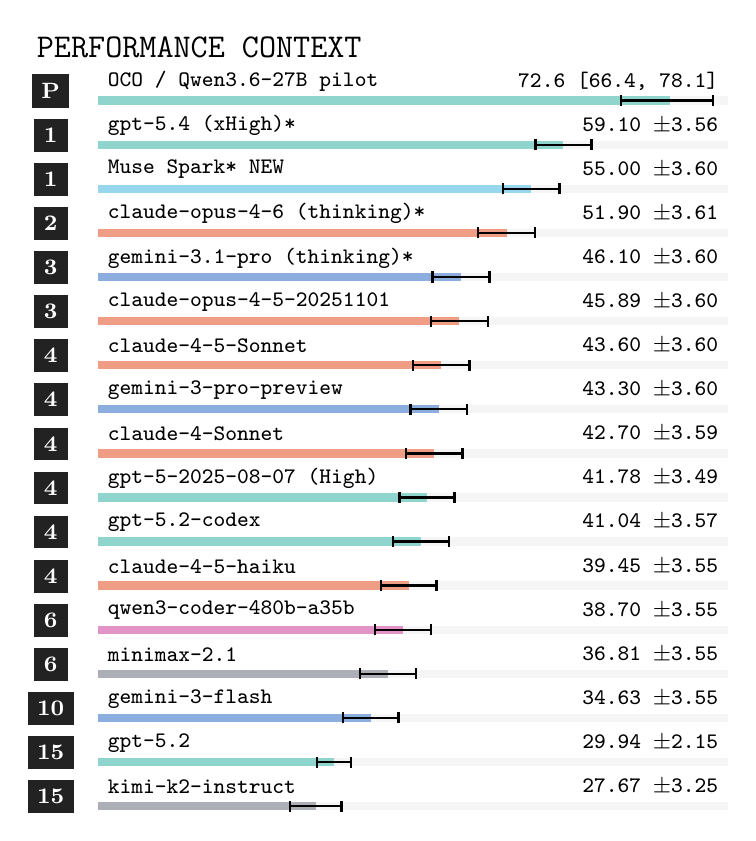
\begin{tikzpicture}[x=0.1cm,y=0.56cm]
\node[anchor=west,font=\large\ttfamily\bfseries] at (-9,17.1) {PERFORMANCE CONTEXT};
\newcommand{\leaderrow}[8]{%
  \node[minimum width=0.43cm,minimum height=0.38cm,fill=ocoDark,text=white,font=\footnotesize\bfseries] at (-6,#1+0.10) {#2};
  \node[anchor=west,font=\footnotesize\ttfamily] at (0,#1+0.32) {#3};
  \node[anchor=east,font=\footnotesize\ttfamily] at (80,#1+0.32) {#8};
  \draw[fill=ocoGray!55,draw=none] (0,#1-0.21) rectangle (80,#1-0.02);
  \draw[fill=#7!72,draw=none] (0,#1-0.21) rectangle (#4,#1-0.02);
  \draw[black,line width=0.85pt] (#5,#1-0.115) -- (#6,#1-0.115);
  \draw[black,line width=0.85pt] (#5,#1-0.24) -- (#5,#1+0.01);
  \draw[black,line width=0.85pt] (#6,#1-0.24) -- (#6,#1+0.01);
}
\leaderrow{16}{P}{OCO / Qwen3.6-27B pilot}{72.6}{66.4}{78.1}{ocoTeal}{72.6 [66.4, 78.1]}
\leaderrow{15}{1}{gpt-5.4 (xHigh)*}{59.10}{55.54}{62.66}{ocoTeal}{59.10 $\pm$3.56}
\leaderrow{14}{1}{Muse Spark* NEW}{55.00}{51.40}{58.60}{scaleSky}{55.00 $\pm$3.60}
\leaderrow{13}{2}{claude-opus-4-6 (thinking)*}{51.90}{48.29}{55.51}{scaleSalmon}{51.90 $\pm$3.61}
\leaderrow{12}{3}{gemini-3.1-pro (thinking)*}{46.10}{42.50}{49.70}{scalePurple}{46.10 $\pm$3.60}
\leaderrow{11}{3}{claude-opus-4-5-20251101}{45.89}{42.29}{49.49}{scaleSalmon}{45.89 $\pm$3.60}
\leaderrow{10}{4}{claude-4-5-Sonnet}{43.60}{40.00}{47.20}{scaleSalmon}{43.60 $\pm$3.60}
\leaderrow{9}{4}{gemini-3-pro-preview}{43.30}{39.70}{46.90}{scalePurple}{43.30 $\pm$3.60}
\leaderrow{8}{4}{claude-4-Sonnet}{42.70}{39.11}{46.29}{scaleSalmon}{42.70 $\pm$3.59}
\leaderrow{7}{4}{gpt-5-2025-08-07 (High)}{41.78}{38.29}{45.27}{ocoTeal}{41.78 $\pm$3.49}
\leaderrow{6}{4}{gpt-5.2-codex}{41.04}{37.47}{44.61}{ocoTeal}{41.04 $\pm$3.57}
\leaderrow{5}{4}{claude-4-5-haiku}{39.45}{35.90}{43.00}{scaleSalmon}{39.45 $\pm$3.55}
\leaderrow{4}{6}{qwen3-coder-480b-a35b}{38.70}{35.15}{42.25}{scalePink}{38.70 $\pm$3.55}
\leaderrow{3}{6}{minimax-2.1}{36.81}{33.26}{40.36}{ocoMute}{36.81 $\pm$3.55}
\leaderrow{2}{10}{gemini-3-flash}{34.63}{31.08}{38.18}{scalePurple}{34.63 $\pm$3.55}
\leaderrow{1}{15}{gpt-5.2}{29.94}{27.79}{32.09}{ocoTeal}{29.94 $\pm$2.15}
\leaderrow{0}{15}{kimi-k2-instruct}{27.67}{24.42}{30.92}{ocoMute}{27.67 $\pm$3.25}
\end{tikzpicture}
\caption{Published SWE-bench Pro performance context from Scale Labs values supplied for this report, with OCO's seeded-subset pilot added as a clearly labeled pilot row. The OCO row is not a leaderboard submission because it uses the seeded-subset submitted-patch denominator; it shows the magnitude of the engineering result against public full-benchmark scores. Whiskers show the reported uncertainty intervals.}
\label{fig:leaderboard}
\end{figure}

\begin{figure}[H]
\centering
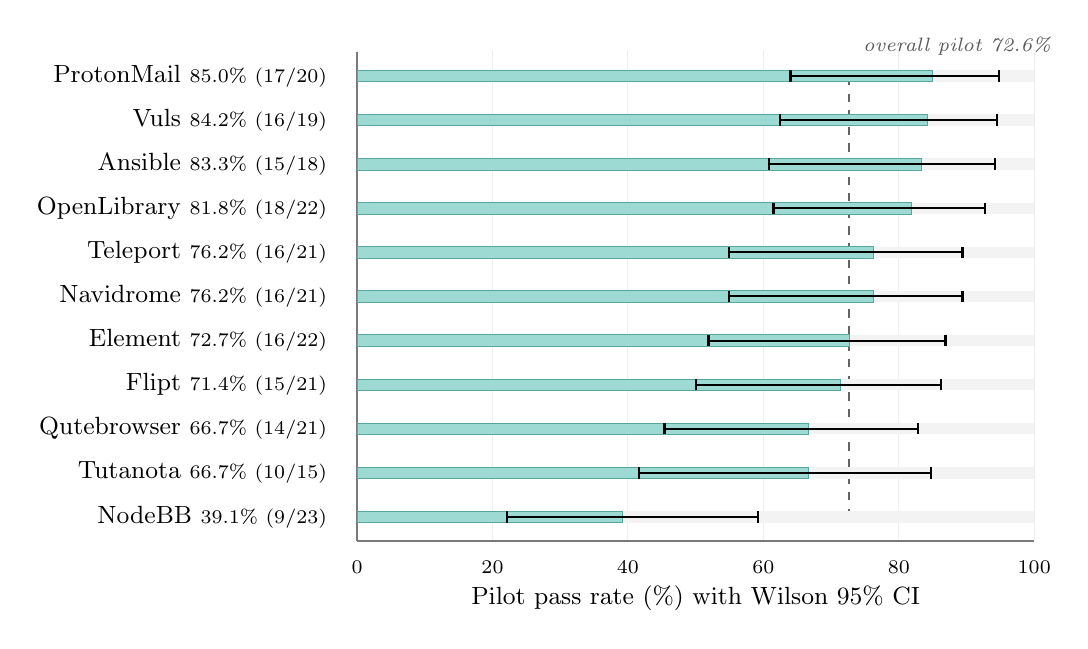
\begin{tikzpicture}[x=0.086cm,y=0.56cm]
\newcommand{\repobar}[6]{%
  \node[anchor=east,font=\small] at (-3,#1) {#2 \scriptsize #3};
  \draw[fill=ocoGray!65,draw=none] (0,#1-0.13) rectangle (100,#1+0.13);
  \draw[fill=ocoTeal!62,draw=ocoTeal!85!black,line width=0.25pt] (0,#1-0.13) rectangle (#4,#1+0.13);
  \draw[black,line width=0.75pt] (#5,#1) -- (#6,#1);
  \draw[black,line width=0.75pt] (#5,#1-0.13) -- (#5,#1+0.13);
  \draw[black,line width=0.75pt] (#6,#1-0.13) -- (#6,#1+0.13);
}
\foreach \x in {0,20,40,60,80,100} {
  \draw[ocoGray!95,line width=0.35pt] (\x,-0.55) -- (\x,10.6);
  \node[font=\scriptsize,anchor=north] at (\x,-0.78) {\x};
}
\draw[ocoDark!60,line width=0.5pt] (0,-0.55) -- (100,-0.55);
\draw[ocoDark!60,line width=0.5pt] (0,-0.55) -- (0,10.55);
\draw[dashed,ocoDark!70,line width=0.65pt] (72.6,0) -- (72.6,10);

\repobar{10}{ProtonMail}{85.0\% (17/20)}{85.0}{64.0}{94.8}
\repobar{9}{Vuls}{84.2\% (16/19)}{84.2}{62.4}{94.5}
\repobar{8}{Ansible}{83.3\% (15/18)}{83.3}{60.8}{94.2}
\repobar{7}{OpenLibrary}{81.8\% (18/22)}{81.8}{61.5}{92.7}
\repobar{6}{Teleport}{76.2\% (16/21)}{76.2}{54.9}{89.4}
\repobar{5}{Navidrome}{76.2\% (16/21)}{76.2}{54.9}{89.4}
\repobar{4}{Element}{72.7\% (16/22)}{72.7}{51.9}{86.9}
\repobar{3}{Flipt}{71.4\% (15/21)}{71.4}{50.0}{86.2}
\repobar{2}{Qutebrowser}{66.7\% (14/21)}{66.7}{45.4}{82.8}
\repobar{1}{Tutanota}{66.7\% (10/15)}{66.7}{41.7}{84.8}
\repobar{0}{NodeBB}{39.1\% (9/23)}{39.1}{22.2}{59.2}

\node[font=\scriptsize\itshape,anchor=south west,text=ocoDark!75] at (73.3,10.25) {overall pilot 72.6\%};
\node[font=\small,anchor=north] at (50,-1.35) {Pilot pass rate (\%) with Wilson 95\% CI};
\end{tikzpicture}
\caption{Per-repository pilot pass rate (162/223 submitted clean patches, current-evaluator replay), sorted by point estimate. Whiskers are Wilson 95\% CIs; per-repo $n=15$--$23$ makes intervals wide. NodeBB sits well below the rest of the field. The dashed line marks the overall pilot rate.}
\label{fig:perrepo}
\end{figure}

\paragraph{Representative passing trajectories.}
Two passing rows were inspected against archived OCO histories. A Navidrome task showed PM, Investigator, and Orchestrator activity; the patch fixed deterministic hashing behavior and replayed tests passed. An OpenLibrary task showed PM investigation, spec writing, Orchestrator delegation, vendor-language serialization edits, and 34 relevant replayed tests passing. These witnesses ground the result in real task-relevant edits rather than bookkeeping artifacts.

\section{Negative Result: Confounded Deployment-Profile Collapse}

A later full 731-task generation run changed several variables at once: H200 hardware, FP8 served checkpoint, MTP-4 speculative decoding, and a new standalone controller path. It generated non-empty patches for all 731 public-split tasks. Official Modal evaluation produced \textbf{208 pass, 310 fail, 213 empty-test outputs}: 28.45\% strict over the full split. Figure~\ref{fig:profiles} shows the contrast directly.

\begin{figure}[H]
\centering
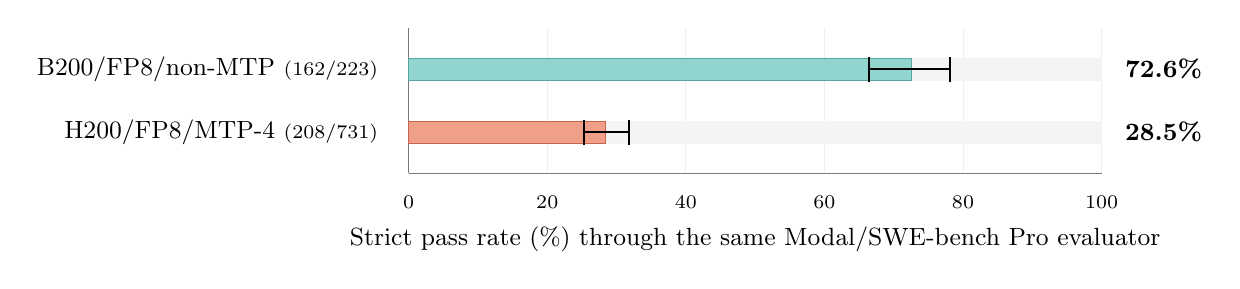
\begin{tikzpicture}[x=0.088cm,y=0.8cm]
\newcommand{\profilebar}[7]{%
  \node[anchor=east,font=\small] at (-3,#1) {#2};
  \node[anchor=west,font=\small\bfseries] at (102,#1) {#3};
  \draw[fill=ocoGray!62,draw=none] (0,#1-0.18) rectangle (100,#1+0.18);
  \draw[fill=#7!70,draw=#7!85!black,line width=0.25pt] (0,#1-0.18) rectangle (#4,#1+0.18);
  \draw[black,line width=0.85pt] (#5,#1) -- (#6,#1);
  \draw[black,line width=0.85pt] (#5,#1-0.2) -- (#5,#1+0.2);
  \draw[black,line width=0.85pt] (#6,#1-0.2) -- (#6,#1+0.2);
}
\foreach \x in {0,20,40,60,80,100} {
  \draw[ocoGray!95,line width=0.35pt] (\x,-0.65) -- (\x,1.65);
  \node[font=\scriptsize,anchor=north] at (\x,-0.85) {\x};
}
\draw[ocoDark!60,line width=0.5pt] (0,-0.65) -- (100,-0.65);
\draw[ocoDark!60,line width=0.5pt] (0,-0.65) -- (0,1.65);
\profilebar{1}{B200/FP8/non-MTP \scriptsize(162/223)}{72.6\%}{72.6}{66.4}{78.1}{ocoTeal}
\profilebar{0}{H200/FP8/MTP-4 \scriptsize(208/731)}{28.5\%}{28.45}{25.3}{31.8}{ocoOrange}
\node[font=\small,anchor=north] at (50,-1.35) {Strict pass rate (\%) through the same Modal/SWE-bench Pro evaluator};
\end{tikzpicture}
\caption{Same model family, same evaluator, two serving/controller profiles. Bars are strict pass rates; whiskers are Wilson 95\% CIs. The intervals do not overlap: the difference is real, but the H200 run changed hardware, speculative decoding, and controller simultaneously, so it does not isolate a single causal variable.}
\label{fig:profiles}
\end{figure}

The low H200 score initially raised the possibility of evaluator or bundle corruption. Three checks pointed back to generation quality: bundle validation found no duplicate, empty-patch, or raw/patch ID mismatch; raw-vs-sanitized evaluation behaved similarly on an unknown-heavy sample; and replaying the earlier B200 patch bundle through the same current evaluator reproduced the high result.

\paragraph{Patch-level witnesses.}
Five old-pass/current-regressed witnesses were inspected patch-by-patch. The current patches failed by ordinary code-quality mechanisms: Flipt had incompatible config/exporter symbols; Navidrome left an expected helper undefined; Vuls missed macOS constants and scanner wiring; Teleport invented a different matcher API; and OpenLibrary changed language serialization into the wrong representation. The H200 FP8 + MTP-4 run is a failed deployment-profile experiment. The actionable lesson: throughput wins are not enough; long-horizon coding agents need task-level quality A/B tests before serving changes are trusted.

\section{Artifact Availability and Reproducibility}

Small artifacts are in this repository: controller code, run notes, result summaries, forensic reports, and this paper. Large bundles and attempt histories are not committed because they contain hundreds of megabytes to many gigabytes of patches, evaluator outputs, and worktrees. Three evidence classes:

\begin{itemize}
  \item \textbf{Checked-in source evidence:} current controller task-source pinning and canonicalization; documentation of result policy and H200 run deviations.
  \item \textbf{Archived local evidence:} old runner source, seeded-250 preparation report, final-223 bundle manifest, attempt histories, and original evaluation outputs under the external archive.
  \item \textbf{Pod/replay evidence:} current Modal replay output roots and H200 raw/sanitized bundle records, including SHA-256 hashes and sanitizer removal manifests.
\end{itemize}

For public release, the strongest next artifact step is to publish compact manifests: selected instance IDs, per-row replay status, excluded artifact-row IDs and reasons, bundle hashes, and witness summaries. This lets readers audit the methodology without downloading full worktrees.

\paragraph{Known artifact-label caveat.}
Legacy filenames and some later notes refer to the positive replay bundle as ``old NVFP4.'' The archived final B200 seeded-250 methodology note records \texttt{Qwen/Qwen3.6-27B-FP8}. This report follows the archived methodology note. Any future public artifact should either recover the original Runpod serving command or rename the legacy replay labels so the quantization description is unambiguous.

\section{Threats to Validity}

\paragraph{No matched baseline.}
The positive pilot lacks a same-model, same-serving mini-SWE-agent or SWE-agent baseline on the exact seeded subset. It is strongest as an engineering pilot and artifact-backed case study.

\paragraph{Subset and non-submission.}
The 250-task subset was deterministic and repository-balanced, but it was still a subset. Only 223 selected rows became submitted clean patch rows. The strict 223-row score measures submitted patch quality; the 250-row conservative score exposes the cost of non-submission.

\paragraph{Evaluator artifacts and manual classification.}
Manual classification of empty-test outputs can introduce judgment. This is why the strict 162/223 number stays primary and the 162/219 artifact-adjusted score is labeled diagnostic.

\paragraph{Audit loop not enforced.}
OCO's Auditor was available but most clean patches did not show an observed Auditor pass. Audit is a runtime feature in this report, not the measured treatment.

\paragraph{Serving/controller confounding.}
The H200 collapse changed hardware, quantization/checkpoint, MTP, controller behavior, prompt/tool surface, and continuation policy. Replay and witness forensics isolate the collapse away from evaluator-only explanations but do not identify a single causal variable.

\paragraph{Agent-assisted benchmark implementation.}
The benchmark harness and documentation were developed with agent assistance. This increases the need for source-backed claims, manifests, hashes, and independent re-runs before any formal publication.

\paragraph{Artifact access.}
Some evidence currently lives in local external storage or pod-local paths. A reader cannot fully reproduce the analysis until compact public manifests and shareable replay artifacts are packaged.

\section{Conclusion}

OCO's seeded-subset pilot shows that a durable orchestration harness can produce strong repository-repair results with open-weight Qwen3.6-27B under an archived B200 non-speculative profile. The failed H200 full run makes the systems lesson sharper: faster serving is not automatically better serving. Harness design, serving profile, and evaluator evidence are first-class experimental variables in coding-agent research.

\bibliographystyle{plain}
\bibliography{references}

\end{document}
